\chapter{Gegenüberstellung}
\thispagestyle{fancy}
\section{Planung}

Das Thema Planung wird unter folgenden fünf Aspekten betrachtet:
\begin{enumerate}
\item Release-Planung
\item Priorisierung
\item Planungssicherheit
\item Planungsaufwand
\item Nachvollziehbarkeit
\end{enumerate}

\subsection{Release-Planung}

Der Aspekt «Release-Planung» wurde gewählt, weil Scrum keine Aussage über die Release-Planung im weiteren Kontext aussagt. Wie wird eine abteilungsübergreifende Planung gemacht? Wie wird das Management informiert? Diese Fragen werden in diesem Kapitel beantwortet.

{\Large Scrum:} \cite{planningReleaseScrum} \medskip

Der Release-Plan ist ein höhergestellter Plan, der mehrere Sprints beinhaltet und während der Release-Planung festgelegt wird. Der Plan definiert welche Features umgesetzt werden und wann diese erfüllt sind. Er dient auch dazu den Fortschritt innerhalb des Projekts verfolgen zu können. Es können mehrere Releases während des Projekts geplant werden oder einfach ein finales Release am Ende des Projekts. \medskip

Um eine Release-Planung durchführen zu können, muss Folgendes bekannt sein:
\begin{itemize}
\item Ein priorisiertes Scrum-Backlog
\item Die Ressourcen des Scrum-Teams
\item Zielerfüllungsbedingungen
\end{itemize}
Ein Release-Plan kann Termin- oder Feature-geführt sein.\smallskip

Bei Termin-geführten Projekten wird spezifiziert, welche Features bis zu einem bestimmten Termin erfüllt werden können.\smallskip

Kommt es bei einem Termin-geführten Projekt zu Verzögerungen, so muss gegebenenfalls der Termin angepasst werden. Dies muss in Abstimmung mit dem Kunden gemacht werden.

Bei Feature-geführten Projekten wird spezifiziert, bis zu welchem Termin das Feature erfüllt ist. Kommt es bei Feature-geführten Projekten zu Verzögerungen, so muss zusammen mit dem Kunden besprochen werden, welche Features gegebenenfalls weggelassen werden können oder entsprechend angepasst werden müssen.\smallskip

Wie der Backlog ist auch der Release-Plan bei Scrum nicht statisch. Dieser kann sich mit dem Backlog ändern oder auch nach jedem Sprint wieder diskutiert und überarbeitet werden.
\bigskip 

{\Large DAD:} \cite{planningReleaseDad} \medskip

In DAD wird die Release Planung initial in der Inception Phase gemacht. Der Leitfaden empfiehlt für die Releaseplanung folgende sechs Fragen zu beantworten:
\begin{itemize}
	\item Wer wird an der Planung beteiligt sein?
	\item Was ist der Umfang unseres Planungsaufwands?
	\item Was ist unsere Gesamtstrategie, die diesen Plan vorantreibt?
    \item Wie detailliert sollte unser Plan sein?
    \item Welche Kadenzen wird das Team annehmen?
    \item Welchen Ansatz zur Schätzung werden wir wählen?
\end{itemize}
Damit soll sichergestellt werden, dass grundlegende Managementfragen gegenüber den Stakeholdern beantwortet sind. Zudem wird erreicht, dass eine durchführbare Strategie besteht und zwischen Stakeholder und Delivery Team ein gemeinsames Verständnis existiert.


\subsection{Priorisierung}

Die «Priorisierung» wurde als Aspekt gewählt, weil wichtig ist wer priorisiert und es wichtig ist das Riskio von Abhängigkeiten zwischen den Aufgaben zu reduzieren bzw. zu vermeiden.

{\Large Scrum:} \cite{planningPrioScrum} \medskip

Das Scrum-Team priorisiert zusammen mit dem Product-Owner die Tasks/Stories aus dem Scrum-Backlog. Wichtig dabei ist, dass nicht nur priorisiert, sondern auch sortiert werden muss. Beim Sortieren wird auch die Reihenfolge von Abläufen berücksichtigt. Die Priorisierung geht mit der Sortierung Hand in Hand. \smallskip

Weiter achtet Scrum auch darauf, dass die wertvollsten Inkremente frühstmöglich umgesetzt werden. Eine Bewertung oder Posteriorisierung von Tasks kann über diverse Verfahren ermittelt werden (z.B. Kano, MoSCoW, usw.). Grundsätzlich werden immer der Nutzen und Aufwand berücksichtigt um eine Einschätzung dazu zumachen. \bigskip 

{\Large DAD:} \cite{planningPrioDad} \medskip

Die Priorisierung bei DAD verhält sich ähnlich wie die Release-Planung. Grundsätzlich gilt das Rolling-Wave-Modell. Das heisst, dass höher priorisierte Features detaillierter spezifiziert werden und tiefer priorisierte nur grob. Die Priorisierung kann jederzeit wieder angepasst werden.


\subsection{Planungsumfang}

Für die Planung ist ausschlaggebend, welchen Umfang für die Planung berücksichtig wird. Das heisst, welche Arbeiten bzw. Aufwände fallen in die Planung oder nicht.

{\Large Scrum:} \medskip

In Scrum betrifft der Umfang immer direkt das Produkt. Der Scope beinhaltet Features ausgedrückt z.B. als User Stories. Diese sind im Scrum-Backlog abgelegt und verwaltet.\medskip

Man kann in Scrum nicht-funktionale Punkte wie Ferien oder Schulungen auch berücksichtigen. Z.Bsp. muss die Kapazität für einen Sprint angepasst werden wenn ein Teammitglied währenddessen im Urlaub ist. Oder Eine Schulung des Betreiber-Teams kann als User-Story erfasst werden. Jedoch sind solche Anforderungen nicht implizit in Scurm angedacht.	
\bigskip 

{\Large DAD:} \cite{planningScopeDad} \medskip

DAD geht hier einen Schritt weiter und definiert nicht nur Features sondern sogenannte Working-Items. Bei denen werden auch nicht-funktionale Anforderungen definiert wie z.B. Schulungen, Ferien, Unterstützung anderer Teams usw.	


\subsection{Planungsaufwand}

Im Rahmen der Planung stellt sich die Frage, welchen Aufwand die Planung braucht. Ist es ein wiederholender Prozess mit immer gleichem Aufwand oder ist es ein einmaliger initialer Prozess.

{\Large Scrum:} \medskip

Der Planungsaufwand von Scrum ist relativ gering und ist im iterierenden Prozess von Scrum bereits integriert. Die Planung wird bei Scrum vor jedem Sprint im sogenannten Sprint Planning gemacht. Dabei werden die zu erledigenden Items definiert. Schlussendlich wird der Umfang des Sprints vom ganzen Team bestätigt.\bigskip 

{\Large DAD:} \medskip

Initial ist der Planungsaufwand bei DAD höher als in Scrum. Man muss nebst der eigentlichen Planung des Produkts auch diverse Analysen von Ist-Zuständen bezüglich Ressourcen und Zuständen innerhalb des Unternehmens machen um die Rahmenbedingungen für das Projekt zu legen.
Dies bringt der Vorteil, dass in einem vielleicht eher unerfahrenen Scrum Team, auch nicht-funktionale Anforderungen berücksichtigt werden. Auch hat so Scrum in einem klassischen Unternehmen mehr Akzeptanz, da es andere Abteilungen und Prozesse berücksichtigt und mit einbezieht. \medskip

Während der Construction Phase ist der Planungsaufwand analog demjenigen von Scrum.


\subsection{Risikomanagement}

Bei jeder Planung stellt sich auch die Frage des Scheiterns. Dieser Aspekt zeigt wie mit den Risiken umgegangen wird.

{\Large Scrum:} \medskip

Bei Scrum wird das Risikomanagement hauptsächlich durch die Kommunikation zwischen dem Kunden und Team geführt. Diese geht über den Product Owner. Dabei muss der Kunde durch seinen stetigen Einfluss mögliche Risiken ausschliessen können. Er kann dies mittels Akzeptanzkriterien beeinflussen.\newline

Aus Team-interner Sicht ist die Definition of Done das Kontrollinstrument, um Qualität aber auch Vollständigkeit sicherzustellen.

Als weiteres Instrument dient die Review am Ende jedes Sprints. An jener werden dem Kunden die umgesetzten Items präsentiert und er kann Einfluss nehmen, sowie Missverständnisse aufdecken und klären.

\bigskip 

{\Large DAD:} \medskip

Um das Risiko von Fehlkommunikation zu verringern werden bei DAD gegenüber Scrum leichte Meilensteine eingeführt, bei denen ein Abgleich mit dem Kunden stattfindet. \medskip

Weiter sieht DAD die Planung von festen Releases vor. Damit soll regelmässig Software zur Verfügung gestellt werden, um ein Feedback des Kunden zu erhalten und frühzeitig festzustellen, ob man die Anforderungen so erfüllen kann. Dies ist gleich wie bei Scrum.

\section{Zusammenarbeit}


Das Thema Planung wird unter folgenden fünf Aspekten betrachtet:
\begin{enumerate}
	\item Koordination im Team
	\item Rolle und Aufgaben des Kunden
	\item Kommunikation im Team
	\item Know-How-Transfer im Team
	\item Organisation in grösseren Teams
\end{enumerate}

\subsection{Koordination im Team}


Die Koordination im Team wurde als Aspekt gewählt, weil es interessiert wie sich ein Team organisiert und welche Methoden/Prozesse vom Vorgehensmodell mitgegeben werden um dies zu fördern. \medskip

{\Large Scrum:} \medskip

Scrum geht grundsätzlich von einer selbstorganisierten Koordination aus. Einzig der Scrum Master hat eine «koordinierende» Rolle, jedoch nur im Bezug auf den Prozess und Schnittstellen ausserhalb des Projekts.
Als wichtigstes Instrument für Koordination in Scrum oder auch allgemein in agilen Vorgehensmodellen dient die Kommunikation mit den anderen Team-Mitgliedern. Dies wird in Scrum mit regelmässigen Treffen/Aussprachen realisiert. Wie zum Beispiel das Daily Stand-up oder Scrum of Scrums (Team übergreifend), welche speziell für die Koordination angedacht sind. Weitere Routinen wie Daily Scrum oder die Reflektion dienen auch der Koordination und deren Verbesserung, auch wenn das nicht primär ihr Ziel ist.
Somit liegt die Verantwortung für die Koordination seiner Aufgaben bei jedem einzelnen Teammitglied selbst.

\bigskip 

{\Large DAD:} \cite{collabCoordInTeamDad} \medskip

DAD möchte, dass folgende Fragen bezüglich Koordination in einem Scrum-Team geklärt sind, um eine effektive Organisation innerhalb des Teams zu haben.
\begin{itemize}
	\item 	Wie werden Informationen innerhalb des Teams ausgetauscht?
	\item 	Wer darf die vom Team erstellten Artefakte aktualisieren? 
	\item 	Wie werden wir uns innerhalb des Teams koordinieren?
	\item 	Falls wir Teil eines größeren Teams sind, wie werden wir dann innerhalb dieses Teams koordinieren?
	\item 	Wie werden wir mit Enterprise-/IT-Teams wie Enterprise Architects und Data Managern zusammenarbeiten?
	\item 	Wie werden wir unsere Release-/Einsatzplanung mit dem Rest des Unternehmens koordinieren?
	\item 	Falls wir geografisch verteilte Teammitglieder haben, wie werden wir dann mit ihnen zusammenarbeiten?
\end{itemize}
Innerhalb des Teams soll also klar definiert sein, mit welchen Routinen (tägliches Treffen, Video-Konferenzen, usw.) Informationen zwischen den Teammitgliedern ausgetauscht werden und welche Tools dazu verwendet werden. Auch soll geregelt sein, wer die finalen Artefakte verwaltet, dass es hier keine Überschneidungen oder Unklarheiten gibt.
Das sind Fragen, welche bei Scrum nicht implizit geklärt werden. Daher können diese Fragen gerade bei eher unerfahren Teams von Vorteil sein.
Innerhalb des Teams soll also klar definiert sein, mit welchen Routinen (tägliches Treffen, Video-Konferenzen, usw.) Informationen zwischen den Teammitgliedern ausgetauscht werden und welche Tools dazu verwendet werden. Auch soll die Zuständigkeit geregelt sein wer die finalen Artefakten verwaltet, dass es hier keine Überschneidungen oder Unklarheiten gibt.
\medskip

Weiter muss gerade bei agilen Teams innerhalb eines Unternehmen auch die Koordination mit anderen Teams/Abteilungen geregelt sein.
\medskip

Was oft vernachlässigt wird, ist die Koordination mit Teammitglieder an anderen geografischen Orten. Der Informationsaustausch wird hier anspruchsvoller, da direkte verbale Kommunikation, welche die effektivste ist, nicht möglich ist.


\subsection{Rolle und Aufgaben des Kunden}

Die Rolle und Aufgabe des Kunden wurde als Aspekt gewählt, weil es interessiert wie der Kunde im Projekt/Prozess miteinbezogen wird. \medskip

{\Large Scrum:} \medskip

Der Kunde soll in Scrum während des ganzen Projekts immer involviert sein. Folgende Möglichkeiten gibt es den Kunden zu involvieren:
\begin{itemize}
	\item Der Kunde wird zum Initial-Meeting eingeladen.
	\item Das Backlog wird zusammen mit dem Kunden verwaltet.
	\item Der Kunde nimmt auch an Reviews teil, um Arbeiten zu besprechen und als abgeschlossen zu definieren.
\end{itemize}
Durch den konsequenten Miteinbezug des Kunden wird das Risiko vermindert, dass der Kunde nicht zufrieden ist. Dies weil er fortlaufend Einfluss nehmen kann und mit seiner Teilnahme auch frühe Schritte/Arbeiten bestätigt.
\bigskip 

\pagebreak
{\Large DAD:} \cite{collabCustomerRoleDad} \medskip

DAD hat bezüglich dem Kunden eine andere auch radikalere Haltung. In DAD will man den Begriff «Kunde» nicht verwenden, sondern nur Stakeholder. Diese werden in folgende Gruppen unterteilt:
\begin{itemize}
	\item Endbenutzer: Personen die das Produkt schlussendlich verwenden.
	\item Vorstehende: Personen die schlussendlich entscheiden, welches Produkt beschafft wird, Bezahlungen freigeben, usw.
	\item Partner: Unterhalter, Betreiber, Entwickler von externen Systemen, Juristen, usw.
	\item Interne: Personen innerhalb des Entwicklungsteams und welche technische oder geschäftliche Dienste liefern
\end{itemize}
Für ein Produkt gibt es nur Stakeholders und es gilt dessen Anforderung genau zu ermitteln und festzulegen. Dazu werden für alle Stakeholder die Bedürfnisse gleichwertig ermittelt und miteinbezogen. \smallskip

Man will also bewusst ein Produkt, das alle Stakeholder gleich berücksichtigt und nicht nur den «bezahlenden Kunden» hauptsächlich priorisiert. Denn nur so wird der Kunde auch ein nachhaltiges und erfolgreiches Produkt erhalten können.

Wichtig ist, dass das Projekt im «wir»-Kontext betrachtet wird und nicht im «ihr»-Kontext. Es gibt nicht den Kunden und das Entwicklungsteam, sondern das Projekt betrifft alle gleich.

\pagebreak

\subsection{Kommunikation im Team}

Die Kommunikation wurde als Aspekt gewählt, da es wichtig ist wie kommuniziert wird um eine effiziente Zusammenarbeit zu gewährleisten, gerade bei geographisch getrennten Teams.\medskip

{\Large Scrum:} \medskip

In Scrum gibt es keine genauere Definieren oder Analyse zur Art der Kommunikation innerhalb des Teams.
\bigskip 

{\Large DAD:} \cite{collabComDad} \medskip

In DAD wird die Kommunikationsart mit ihrem Informationsgehalt gegenübergestellt. Grundsätzlich ist eine Kommunikation von Angesicht zu Angesicht am effizientesten. Jedoch müssen auch andere Faktoren und Anforderungen dabei berücksichtigt werden. Zum Beispiel kann man bei geographisch weit unterschiedlichen nur schwer und teuer regelmässig eine Austausch Angesicht zu Angesicht halten. Da ist man auf eine Anruf oder Email angewiesen. Auch müssen gewisse Kommunikationen aus rechtlichen gründen auch schriftlich festgehalten werden. \medskip

Zusätzlich wird aber auch erwähnt, dass eine grössere Diversität in der Art der Kommunikation auch förderlich für einen effizienten Austausch sein kann.

\begin{figure}[H]
	\centering
	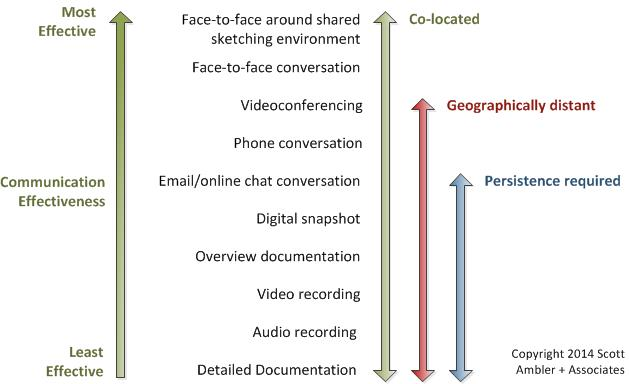
\includegraphics[scale=0.8]{DAD-communicationstechniques}
	\caption{DAD Kommunikationstechniken}
	\label{fig:DAD-communicationstechniques}
\end{figure}

\subsection{Know-How-Transfer im Team}

Know-How-Transfer im Team wurde als Aspekt gewählt, weil hier zu DAD spannende Ideen bringt um Know-How und Kompetenzen in verschiedensten Weisen auszutauschen. \medskip

{\Large Scrum:} \medskip

Scrum macht direkt keine Vorschläge zum Austausch von Know-How. In den Reviews kann ein gewisser Austausch über Know-How statt finden, jedoch ist dort der Fokus primär auf die Zusammenarbeit gerichtet.

\bigskip 

{\Large DAD:} \cite{collabKHTransDad} \medskip

DAD macht einige Vorschläge wie Teammitglieder sich gegenseitig Know-How oder Kompetenzen vermitteln können. \medskip

Folgende Methoden werden vorgeschlagen:
\begin{itemize}
	\item Training, sich etwas beibringen lassen
	\item Open Space, gemeinsam über Fragestellungen diskutieren
	\item Non-Solo work, also bewusst arbeiten nicht alleine machen
	\item Mentoring, sich von jemandem etwas erklären lassen
	\item Hackathons, gemeinsam in z.B. einem Tag mal eine Applikation für andere Anwendung entwickeln.
	\item Communities of Practice, Personen aus verschiedenen Abteilungen, welche ähnliche Problemstellungen im Berufsalltag haben.
\end{itemize}

Mit solchen Methoden kann spielerisch und immer wieder in einzelnen Blöcken Know-How und Kompetenzen zwischen den einzelnen Mitarbeitern ausgetauscht werden. Weiter können solche Anlässe auch einen Team-bildenden Effekt haben.


\subsection{Organisation in grösseren Teams}

Die Organisation in mittleren bis grossen Teams wurde als Aspekt gewählt, weil Scrum hier eine Limitierung von max. 7-9 Leuten hat. Es interessiert welchen Ansatz DAD bringt um agile Vorgehensmodelle wie Scrum auch in grösseren Teams anzuwenden.

{\Large Scrum:} \cite{collabollabOrgLargerTeamsScrum} \medskip

Scrum geht von einer maximalen grösse eines Teams von 7-9 Mitgliedern aus. Danach wird das Projekt mit all seinen Prozessen zu lange und ineffizient (z.Bsp. Daily Scrum nicht mehr in 15min möglich). \smallskip

Es wird  dann eine Aufteilung des Teams empfohlen und das Projekt entsprechend zu modularisieren. Um einen Austausch zwischen diesen Teams zu haben soll übergeordnetes Scrums of Scrums gehalten werden, wo nur die einzelnen Product Owner und Scrum Master teilnehmen um ihre Teams zu vertreten.
\bigskip 

{\Large DAD:} \cite{collabollabOrgLargerTeamsDad} \medskip

DAD unterscheidet zwischen kleinen (2-15 Personen )mittleren(15-35 Personen) und grossen (35+ Perosnen) Teams. \medskip

Kleine Teams werden wie Beschrieben in Kapitel 2.3 geführt. Also grundsätzlich Scrum mit zusätzlichen Rollen. \medskip

Mittlere Teams analog zu Scrum of Scrums mit einzelnen Sub-Teams geführt.

Grosse Teams werden in DAD zusätzlich definiert. Hierzu wird zu den einzelnen Subteams ein Leadership Team eingeführt. Dieses enthält folgende zusätzlichen Rollen:
\begin{itemize}
	\item Program Manager: hat die Koordination über das ganze Projekt und das Leadership Team
	\item Product Coordination: Koordiniert alle Team Leader aus den Sub-Teams
	\item Product Ownership: Koordiniert alle Product Owner aus den Sub-Teams
	\item Architecture Ownership: Koordiniert alle Achitecture Owner aus den Sub-Teams
\end{itemize}

Das Leadership Team soll die einzelnen Sub-Team und die Rollen-Inhaber in ihren Tätigkeiten unterstützen und die Koordination zwischen den Teams sicherstellen und unterstützen. 

\section{Zuständigkeit}

Das Thema Zuständigkeiten wird unter folgenden fünf Aspekten betrachtet:
\begin{enumerate}
\item Zuständigkeiten im Team
\item Rollen im Team
\item Verantwortlichkeiten
\item Zielerfüllung
\item Rollenkonflikte
\end{enumerate}

Auf den Aspekt «Zuständigkeiten im Team» wird nicht explizit eingegangen. Die Zuständigkeiten im Team sind über die weiteren viere Aspekte verteilt zu betrachten.

\subsection{Rollen im Team}\label{rollen}

Der Askpekt «Rollen im Team» wurde gewählt, dass für den Prozess ausschlaggebend ist, wer am Prozess beteiligt ist. Welche Rollen gibt es im jeweiligen Prozess und welche Funktion wird der jeweiligen Rolle zugewiesen?

{\Large Scrum:} \cite{scrumRoles} \medskip

In Scrum gibt es drei Rollen, siehe Abbildung \ref{fig:scrumrollen}. Den Scrum Master, den Product Owner und die Team Member. 
\begin{figure}[H]
	\centering
	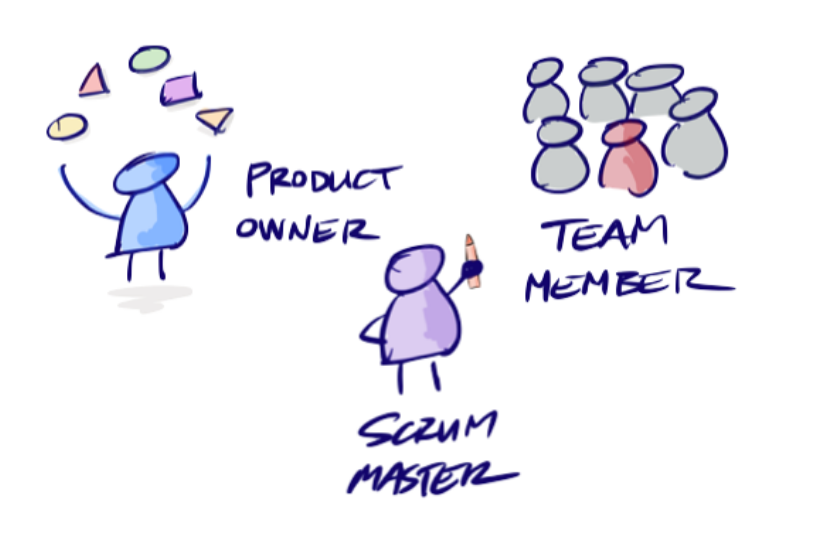
\includegraphics[scale=0.8]{scrum_roles}
	\caption{Scrum Rollen \cite{scrumRoles}}
	\label{fig:scrumrollen}
\end{figure}

Der \textbf{Product Owner} ist die Ansprechperson für Kunden und Stakeholder. Er nimmt die Anforderungen entgegen, priorisiert diese und gibt diese an das Team weiter. Der Product Owner kann aber auch direkt der Kunde sein. In beiden Fällen vertritt er aber die fachliche Sicht, beurteilt die Qualität, Usability und Performance. \medskip

Der \textbf{Scrum Master} dient dem Scrum Team um die gewünschte Performance zu erreichen. Er ist verantwortlich, dass der Prozess zielgerichtet ausgeführt werden kann. Er nimmt sich Problemen, sogenannten Impediments, an und löst diese - mit oder ohne Team. Der Scrum Master fördert den Fortschritt des Teams und lenkt dieses, falls der Fortschritt nicht wie geplant vorankommt. Zudem organisiert er die Scrum Zeremonien - Retrospektive, Review-Meeting, Daily Standups - und sorgt für den Informationsfluss zwischen Team und Product Owner. Er ist sozusagen die gute Seele des Teams. \medskip

Das \textbf{Scrum Team}, oder kurz Team, ist das zentrale Element im Scrum Prozess. Es setzt die Anforderungen um. In Scrum besteht ein Team aus fünf bis zehn Personen. Grössere Teams sollten in mehrere unabhängige Teams aufgetrennt werden. Sehr wichtig bei Scrum ist, dass das Team selbstorganisiert ist. Es bestimmt schlussendlich selbst welche Anforderungen es im Sprint umsetzen will. Dabei beachtet es, dass es am Ende jedes Sprints ein «Increment of  Potentially Shippable Functionality» liefert. In einem Scrum Team sind immer die Disziplinen vorhanden, welche es für das Erreichen des Ziels benötigt.
\bigskip

\pagebreak
{\Large DAD:} \cite{dadRoles} \medskip

Im Gegensatz zu Scrum werden in DAD zusätzliche Rollen definiert, siehe Abbildung \ref{fig:dadrollen}. In DAD werden einzelne Zuständigkeiten explizit aufgeführt, welche in Scrum im Team vereint werden. DAD verwendet gewisse Rollen die auch Scrum verwendet (Team Member und Product Owner), aber unterscheidet hierbei primäre und unterstützende Rollen. Zu den primären Rollen zählen Team Lead, Product Owner, Team Member, Architecture Owner und Stakeholder. Zu den unterstützenden Rollen zählen Spezialisten, Independent Tester, Domänen-Experten, Technische Experten und Integratoren.

\begin{figure}[H]
	\centering
	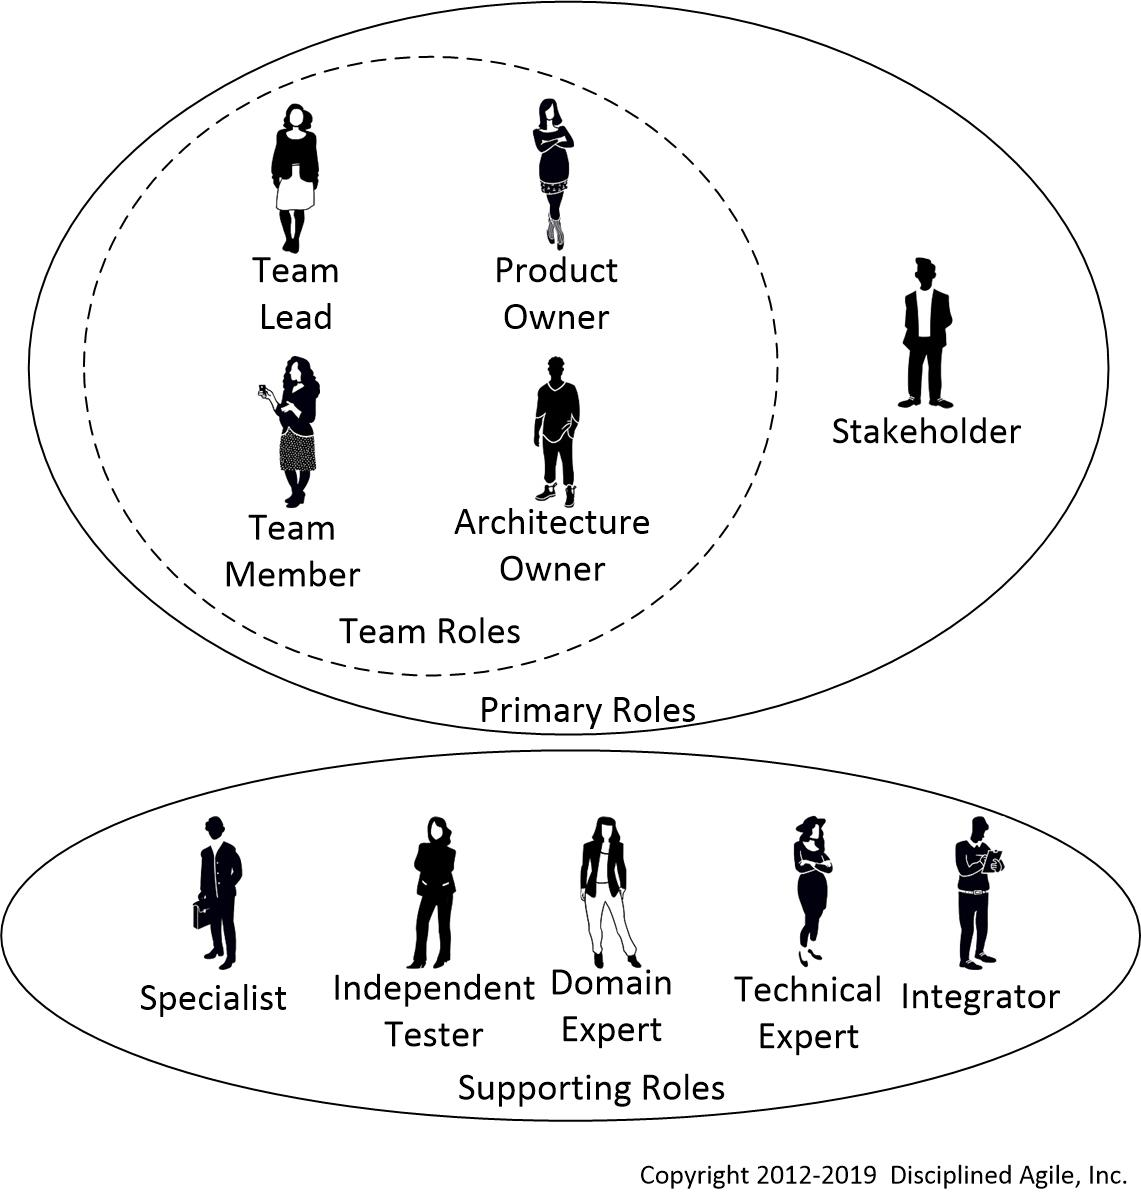
\includegraphics[scale=0.8]{DAD-Roles}
	\caption{DAD Rollen \cite{dadRoles}}
	\label{fig:dadrollen}
\end{figure}

DAD wurde somit stark auf die Bedürfnisse von Unternehmen weiterentwickelt um Anforderungen aus den bestehenden Firmenstrukturen mit Prozessen, Programmen und Rollen anzuwenden. DAD unterstützt mit den sehr spezifischen Rollen insbesondere hierarchische Unternehmensstrukturen.
\bigskip


In diesem Punkt unterscheiden sich die zwei Methoden wesentlich. Warum hat Scrum drei Rollen, DAD hingegen zehn? Scrum konzentriert sich hauptsächlich auf Führungs- und Change-Management-Aspekte während der Konstruktion und hat daher Rollen, die dies widerspiegeln. DAD hingegen konzentriert sich explizit auf den gesamten Delivery Lifecycle und alle Aspekte der Lösungsbereitstellung, einschließlich der technischen Aspekte, die Scrum auslässt. Mit einem grösseren Umfang kommen also mehr Rollen hinzu. Weil DAD beispielsweise Fragen der agilen Architektur umfasst, beinhaltet es auch eine Rolle des Architecture Owners. Scrum adressiert keine Architektur und beinhaltet auch keine solche Rolle.

\subsection{Verantwortlichkeiten}

In diesem Aspekt wird beschrieben wie die Verantwortlichkeiten auf die Rollen verteilt sind und welche Verantwortlichkeiten im Prozess wahrgenommen werden müssen.

{\Large Scrum:}\cite{scrumResponsibilites} \medskip

In Scrum hat jede Rolle ihre Verantwortlichkeit im Prozess. Der Scrum Master hat in erster Linie die Verantwortung zur Einhaltung des Prozesses und der Scrum Spielregeln. Wie bereits im Kapitel \ref{rollen} beschrieben, hat er die Verantwortung zur Beseitigung von Hindernissen.

Der Product Owner hat die Verantwortung die Vision und Wünsche des Kunden an das Team weiterzugeben. Er ist die Stimme der Stakeholder und somit verantwortlich die Bedürfnisse des Kunden zu identifizieren.

Die grösste Verantwortung wird jedoch dem Team zugeteilt. Es legt den Umfang fest, welchen es umsetzt - das sogenannte Sprint Goal. Es verpflichtet sich dazu das Sprint Goal umzusetzen. Bei Problemen oder Störungen muss das Team zeitnah mit dem Kunden bzw. mit dem Product Owner in Kontakt treten, um gegebenenfalls das Sprint Goal anzupassen. Da das Team selbstorganisiert ist, liegt es in seiner Verantwortung, wie das Ziel erreicht wird.

\smallskip
{\Large DAD:}\cite{dadResponsibilites} \medskip

Da es in DAD mehr Rollen als in Scrum gibt, sind auch die Verantwortlichkeiten expliziter.
Wir gehen hier nur auf die Verantwortlichkeiten der primären Rollen ein.

Der Team Lead hat in DAD eine ähnliche Funktion und Verantwortlichkeiten wie der Scrum Master. Er dient dem Team als Coach. Er schaut, dass das Team performant arbeiten kann und fördert das Team in der Verbesserung ihrer Arbeitsweise.

Der Product Owner in DAD unterscheidet sich kaum vom PO in Scrum. Auch in DAD ist er die Stimme des Kunden. Er priorisiert die Aufgaben und versucht die Fragen des Teams zu beantworten oder leitet diese an den Kunden weiter.

Der Architecture Owner ist verantwortlich für die Umsetzung der architektonischen Entscheide. Er trifft die Architektur Entscheide, erstellt das Design der Gesamtlösung und übernimmt die Weiterentwicklung davon. Oft ist der Architecture Owner auch der Lead Entwickler. Manchmal wird er auch Softwarearchitekt oder Solutionarchitekt genannt. Der AO ist keine hierarchische Rolle. Er arbeitet mit dem Team und trifft die Entscheidungen in Absprache mit ihm.

Wie in Scrum hat auch das Team in DAD die grösste Verantwortung. Darunter zählen:

\begin{itemize}
	\item Eine Lösung zu finden, die den Bedürfnissen der Stakeholder entspricht.
	\item Optimierte Nutzung der Ressourcen
	\item Bereitschaft zu einer umfassenden Zusammenarbeit innerhalb Ihres Teams, auch ausserhalb Ihres Fachgebiets.
	\item Informationsaustausch über alle Arbeiten, die im Gange sind.
	\item Andere in Ihren Fähigkeiten und Erfahrungen zu coachen.
	\item Erweiterung Ihrer Kenntnisse und Fähigkeiten ausserhalb Ihres Fachgebiets.
	\item Teilnahme an den Meetings.
	\item Proaktiv nach Wegen zur Verbesserung der Teamleistung suchen
	\item Vermeiden, dass Arbeiten außerhalb der aktuellen Iteration ohne Zustimmung des Teams angenommen werden.
	\item Arbeit so früh wie möglich validieren und mit anderen zusammenzuarbeiten
\end{itemize}

Diese Punkte sind ziemlich Deckungsgleich wie jene die im agilen Manifest geschildert werden. 

\subsection{Zielerfüllung}

In jedem Projekt ist die Zielerreichung das Wesentlichste. Darum wird in diesem Aspekt erläutert wie in beiden Modellen die Zielerreichung bzw. Zielerfüllung sichergestellt wird.

\medskip
{\Large Scrum:}\cite{scrumAC} \medskip

Jedes Artefakt, welches in einer Iteration (Sprint) umgesetzt wird, wird durch Akzeptanzkriterien beschrieben. Diese werden zusammen mit oder durch den Kunden definiert. Anhand dieser Akzeptanzkriterien wird ein Artefakt gemessen. Die Akzeptanzkriterien dienen dem Team, nebst einer genauen Beschreibung des Artefakts, zur Erreichung des Sprint Ziels.

In Scrum wird nach jedem Sprint die sogenannte Review gemacht. Hier wird dem Kunden das Produkt bzw. die umgesetzten Artefakte präsentiert. Hier hat der Kunde die Möglichkeit lenkend einzugreifen. Da in Scrum in kurzen Iterationen gearbeitet wird, kann der Kunde schnell und zeitnah Einfluss auf Missverständnisse nehmen.

Das Team definiert zudem die Definition of Done. Die DoD definiert, wann ein Task abgeschlossen ist. Diese Kriterien müssen nicht zwingend deckend zu den Akzeptanzkriterien sein. Oft hat die DoD umfassendere Punkte wie bspw. Tests, Dokumentation, Review etc.

\medskip

\pagebreak
{\Large DAD:}\cite{processGoals} \medskip

Grundsätzlich hat DAD dieselben Mechanismen zur Sicherstellung der Zielerreichung wie Scrum. Nach jeder Iteration wird, wie in Scrum auch, die Iteration zusammengefasst. Den Stakeholdern wird eine Demo der umgesetzten Tasks gezeigt und es wird entschieden ob man mit dem Vorgehen weitermacht. Zum Abschluss wird eine Analyse über den Way of Work gemacht und die nötigen Verbesserungen werden angebracht.

In DAD wird zudem eine gemeinsame Vision mit den Stakeholdern erstellt. Dies ist ein weiteres Mittel zu Sicherstellung der Zielerreichung.

In DAD besteht jede Phase, Inception, Construction, Transition, aus mehreren Goals, dargestellt in Abbildung \ref{fig:goals}. Ein Goal kann einmal oder mehrmals durchlaufen werden. Ein Goal besteht aus einem oder mehreren Decision Points.

\begin{figure}[H]
	\centering
	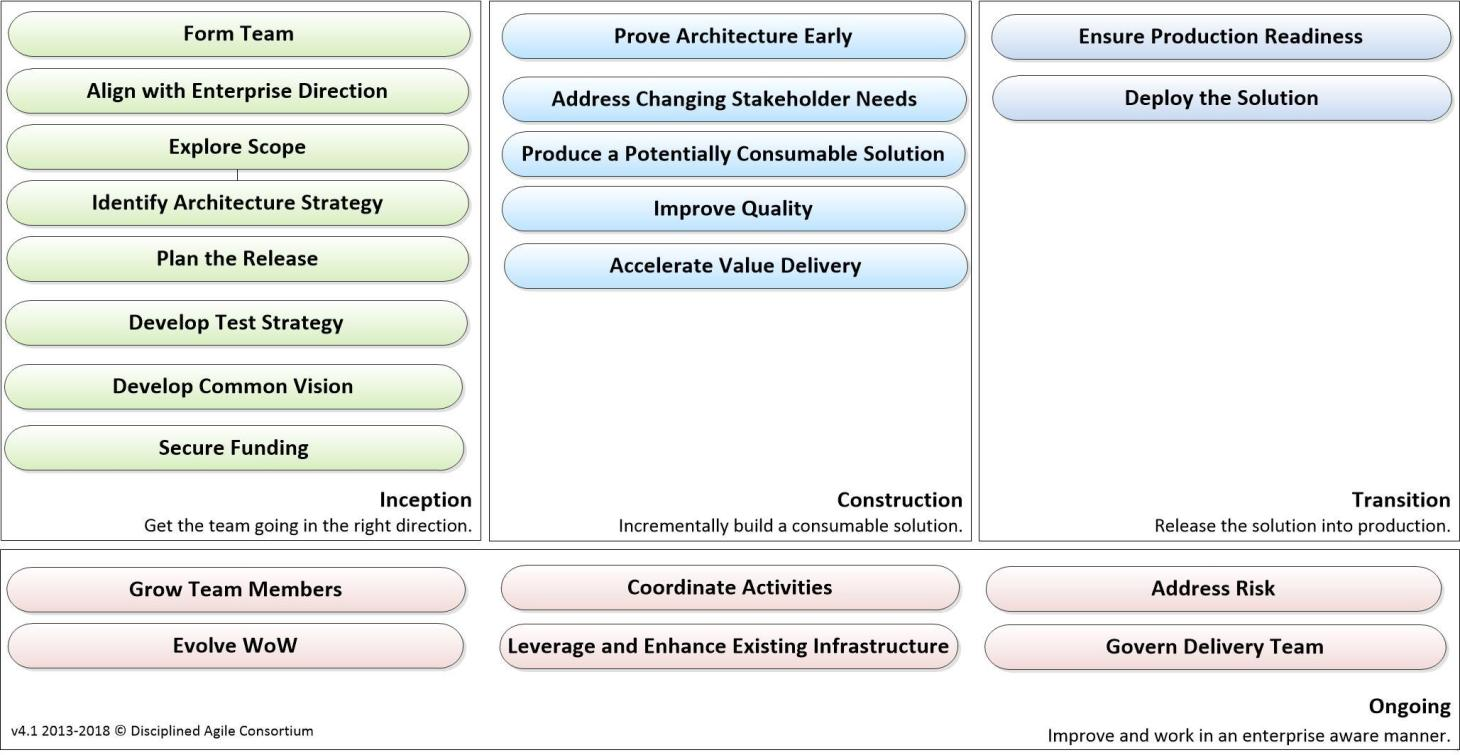
\includegraphics[width=\textwidth]{Lifecycle-Goals.jpg}
	\caption{Lifecycle Goals \cite{processGoals}}
	\label{fig:goals}
\end{figure}

Die Decision Points und Goals dienen der Sicherstellung des Prozesses und somit auch der Erreichung der Ziele.

\subsection{Rollenkonflikte}

Wo es Rollen gibt, gibt es auch Potential für Konflikte. Darum wird unter dem Aspekt «Rollenkonflikte» ausgeführt, wo es in den Modellen Konflikte geben kann \cite{rollenKonflikte}

In Scrum wie auch in DAD sind die Teams selbstorganisiert, was impliziert, dass Hierarchien in Frage gestellt werden. Gerade in Scrum werden explizite Disziplinen nicht gesucht. Scrum fordert, dass alle Mitglieder eines Teams möglichst jede Aufgabe im Sprint abarbeiten können. Ein exklusiver Tester, Programmierer oder Architekt passt somit nicht optimal in ein Scrum Team. Ein gutes Team kann dies aber berücksichtigen und die Nachteile kompensieren. Dies sollte aber wenn möglich in erfahrenen Teams gemacht werden.

DAD bietet hier Unterstützung indem zusätzliche Rollen explizit adressiert werden. So ist nicht nur der Architecture Owner explizit aufgeführt, sondern DAD weist auch unterstützende, sogenannte Supporting Roles, auf. Diese können je nach Bedürfnis des Teams und des Projekts verwendet werden. So kann bei Bedarf ein Tester oder ein Domänen Experte hinzugezogen werden. DAD versucht hier die Rollenkonflikte zu mindern. Jedoch ist darauf hinzuweisen, dass auch DAD Hierarchien in Frage stellt und somit selbstorganisierte Teams fördert.




	